\chapter{\label{chap:ai}Algoritmos de Inteligência Artificial para Elevadores}

A busca pela solução do problema de atribuir elevadores para atender chamadas
feitas pelos passageiros, minimizando alguma métrica, é apresentada pela
literatura pesquisada na forma de alguns algoritmos~\cite{KOEHLEROTTIGER02}.
Tais algoritmos possuem complexidades distintas, indo desde algoritmos triviais,
que sequer podem ser classificados como algoritmos de Inteligência
Artificial~-~mas ainda interessantes para fins de comparação~-, até soluções
mais complexas, onde mais dados são utilizados de modo a tomar decisões mais
complexas.

Em um hipotético cenário ideal, ter-se-ia todos os dados de cada
passageiro~-~\textit{i.e.} cada pessoa que chegasse ao andar informaria de
antemão para qual andar deseja ir antes mesmo de entrar no elevador. No entanto,
isto não é realista no contexto dos sistemas de elevadores instalados
atualmente, onde cada pessoa apenas informa se deseja subir ou descer. Portanto,
os algoritmos aqui descritos tentam fazer inferências e
abstrações\footnote{\textit{e.g.} A lotação do elevador pode ser estimada com
base no peso reportado pela balança interna do elevador, que já se encontra nele
por motivos de segurança, ou abstrair a capacidade e lotação em número de
pessoas.} a respeito de dados que não possuem, quando relevante, ou tentam tomar
decisões ignorando os dados que não estão disponíveis.

A seguir são descritos, do mais simples ao mais complexo, os algoritmos
selecionados para o desenvolvimento na segunda etapa deste trabalho.

\section{\label{sec:ai:nn}Nearest Neighbour}

O algoritmo de \textit{Nearest Neighbour} é o mais ingênuo de todos, e servirá
de base para a avaliação dos demais algoritmos. Seu funcionamento é trivial: o
elevador mais próximo da chamada sempre atenderá esta
chamada~\cite{Friese20061908}. Um dos problemas deste algoritmo é que ele pode
causar muitas mudanças de direção de um elevador, o que acarreta um tempo de
espera maior para os passageiros que estão dentro dele.

Considere, por exemplo, o cenário da figura~\ref{fig:elevadores:nn:bad}. Este
cenário é composto por um prédio de 8 andares com 3 elevadores. A situação dos
elevadores é a seguinte:

\begin{itemize}
\item $E1$ no sexto andar, com ocupação\footnote{A ocupação do elevador é representada pelo percentual dentro do círculo.} de 20\% e como destino\footnote{O destino do elevador é representado pela seta.} o segundo andar;
\item $E2$ no primeiro andar, com ocupação 10\% e como destino o sexto andar;
\item $E3$ no quarto andar, com ocupação 90\% e como destino o sétimo andar.
\end{itemize}

Neste instante, uma nova chamada de corredor é originada no sétimo andar.

\begin{figure}[htb!]
  \centering
  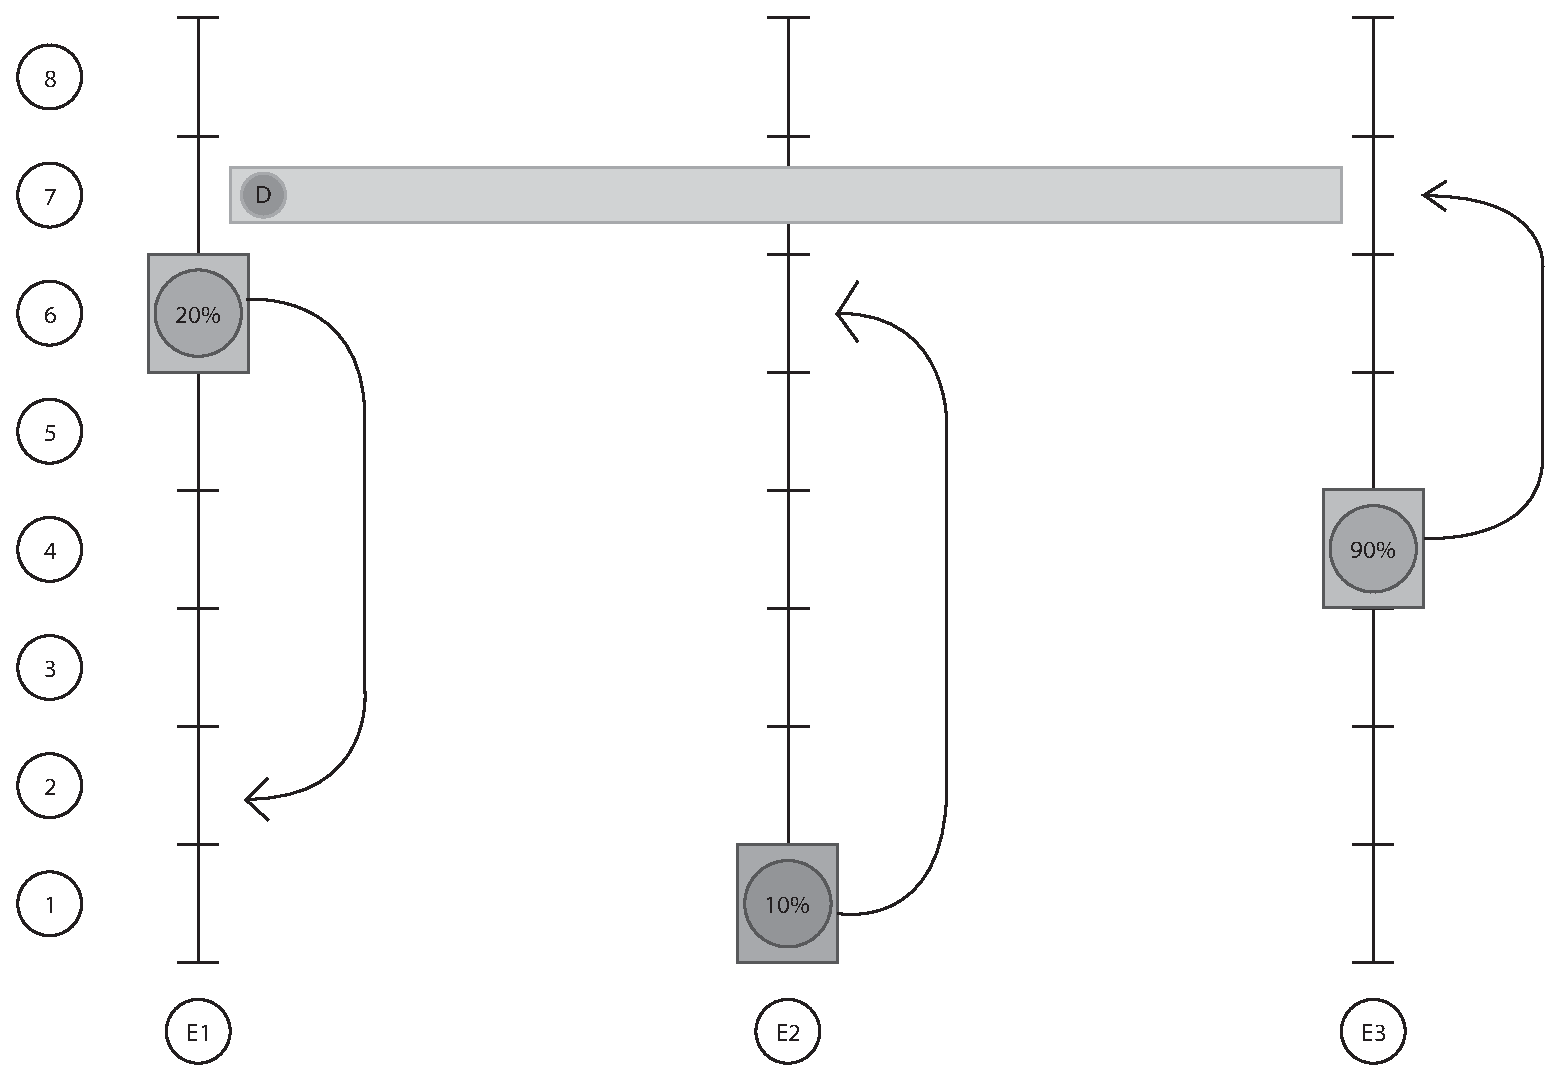
\includegraphics[scale=0.6]{img/elevator_example_nn_bad.eps}
  \caption{Cenário exemplo \#1 de prédio com 8 andares e 3 elevadores.}
\label{fig:elevadores:nn:bad}
\end{figure}

Caso o algoritmo de \textit{Nearest Neighbour} seja utilizado, o elevador $E1$
seria selecionado para atender a chamada no sétimo andar. Isto é claramente ruim
para os passageiros deste elevador. Além disto, é possível notar que o elevador
$E3$ já tinha uma parada programada no sétimo andar e seria possível atender a
chamada sem alterar a agenda de nenhum elevador. O algoritmo de \textit{Nearest
Neighbour}, no entanto, não leva em consideração estas informações.

O único propósito deste algoritmo é servir de base de comparação com outros
algoritmos propostos, de modo a validarmos o simulador. Espera-se que uma
melhora clara de desempenho seja notada ao comparar-se este com o próximo dos
mais triviais, o \textit{Nearest Neighbour Melhorado}.

\section{\label{sec:ai:nnm}Nearest Neighbour Melhorado}

Uma melhoria que pode ser feita ao algoritmo de \textit{Nearest Neighbour} é
considerar o sentido em que o elevador está indo para atender a
chamada~\cite{Friese20061908}. Isto implica em considerar-se agora a informação
de sentido das chamadas. É importante notar que ainda não se considera quantas
pessoas fizeram uma chamada~-~apenas sabe-se que há chamadas no andar, e como
destinos tem-se ``subir'', ``descer'' ou ``ambos''.

Este algoritmo resolve o problema de mudanças de direção que o algoritmo de
\textit{Nearest Neighbour} sofre.

Considere, novamente, o caso ilustrado pela figura~\ref{fig:elevadores:nn:bad}.
Este algoritmo considerará apenas os elevadores que estão parados ou indo no
sentido de onde a chamada foi originada. Neste caso, apenas os elevadores $E2$ e
$E3$ serão considerados. O elevador $E3$ está mais próximo da chamada, então
será escolhido.

No entanto, sua escolha para este trabalho também se dá para fim de comparação
com os outros e validação do simulador. Como seu comportamento é diferente do
caso mais trivial, mas ainda assim bastante simples, poderá ser visto com clareza
algum tipo de melhora no tempo de resposta do sistema simulado, bem como a validade do simulador.

\section{\label{sec:ai:minimize-cost-function}Minimização da Função de Custo}

O primeiro algoritmo de IA a ser testado é simples: define-se uma
função de custo, inerente a cada elevador, que descreve quão custoso
é atender uma chamada, comparado a não atendê-la~\cite{Friese20061908}.
A decisão de qual elevador é escolhido para atender a chamada é feita com base
em qual deles terá o menor valor da função de custo.

Um exemplo de função de custo é:

\[
  J(e, l, p) = \lambda l(p - e)
\]

Onde:
\begin{description}[leftmargin=!,labelwidth=\widthof{\bfseries Pu}]
\item[$\boldsymbol{e}$] Número do andar onde o elevador se encontra
\item[$\boldsymbol{l}$] Percentual de ocupação do elevador
\item[$\boldsymbol{p}$] Número do andar onde a chamada foi originada
\item[$\boldsymbol{\lambda}$] Fator de multiplicação, que assume os seguintes valores:
  \begin{itemize}
    \item $0$, caso o programa atual do elevador faça com que ele passe por
      aquele andar;
    \item $1$, caso o elevador não tenha um programa (\textit{i.e.},
      ele esteja ocioso) ou o elevador esteja indo na direção da chamada;
    \item $2$, caso ele mude de direção para atender esta chamada\footnote{Multiplica-se
        a distância por dois pois é necessário ir até o andar da chamada e então
        voltar para o andar onde se estava anteriormente, para só então atender
        a chamada.}.
  \end{itemize}
\end{description}

\begin{figure}[htb!]
  \centering
  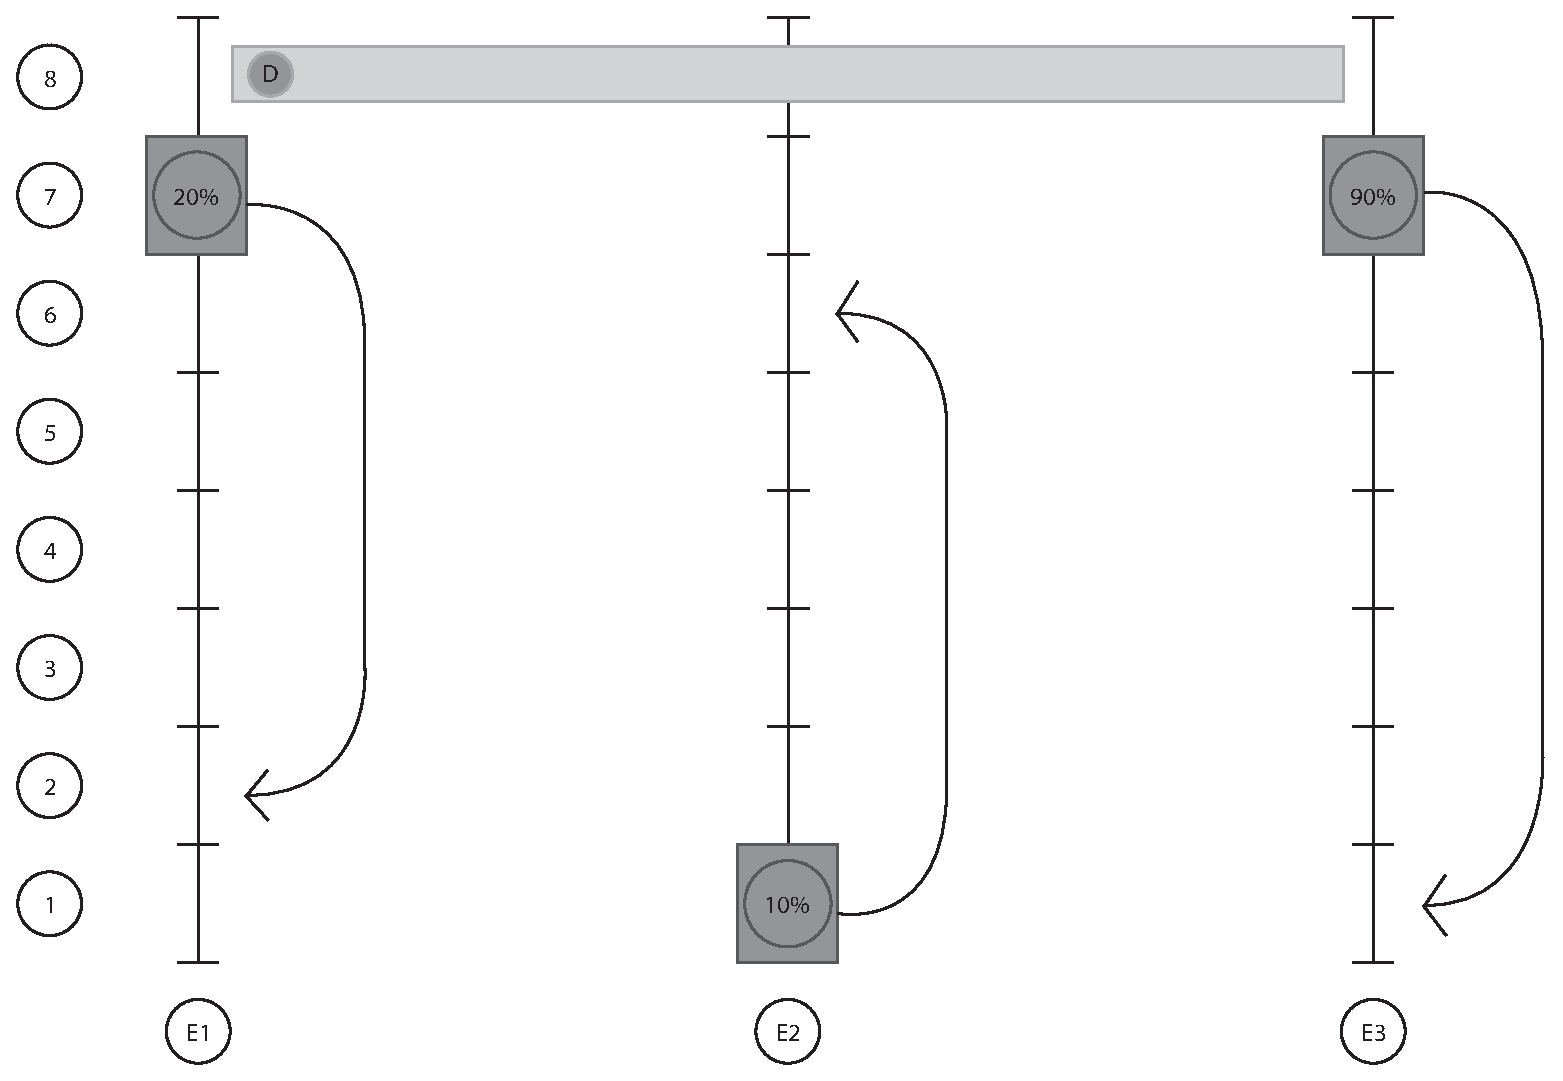
\includegraphics[scale=0.6]{img/elevator_example1.eps}
  \caption{Cenário exemplo \#2 de prédio com 8 andares e 3 elevadores.}
  \label{fig:elevadores-1}
\end{figure}

Utilizando como exemplo o cenário da figura~\ref{fig:elevadores-1}, onde uma
chamada de corredor para descer\footnote{O sentido da chamada é representado
pelo círculo com um \textbf{D}, de \textit{Down}.} é originada no oitavo andar.
A situação de cada elevador é a seguinte:

\begin{itemize}
\item $E1$ no sétimo andar, com ocupação de 20\% e como destino o segundo andar;
\item $E2$ no primeiro andar, com ocupação 10\% e como destino o sexto andar;
\item $E3$ no sétimo andar, com ocupação 90\% e como destino o primeiro andar.
\end{itemize}

Podemos calcular o custo de atender a esta chamada para cada elevador do prédio.
Para o Elevador $E1$:

\[J(7, 0.2, 8) = 2 \times 0.2 \times (8 - 7) = 0.4\]

Neste caso, $\boldsymbol{\lambda}$ é 2, pois o elevador deverá mudar de sentido
(\textit{i.e.}, ele deverá subir até o oitavo andar e então voltar para o sétimo
andar, o que representa um deslocamento de dois andares).

Para o Elevador $E2$:

\[J(1, 0.1, 8) = 1 \times 0.1 \times (8 - 1) = 0.7\]

Neste caso $\boldsymbol{l}$ é $0.1$, pois sua lotação é 10\%\footnote{Como não
há informações a respeito do futuro, não é possível considerar alterações na
carga de um elevador.}, e $(p - e)$ é $7$, pois o elevador deverá subir sete
andares\footnote{Pela regra de cálculo, foi considerada apenas a posição atual
do elevador, e não a posição que ele estará ao fim de sua última atividade.
Seria possivel alterar esta regra, gerando uma função de custo levemente
diferente, com resultados diferentes. É um teste válido para a implementação.}.

Para o Elevador $E3$:

\[J(7, 0.9, 8) = 2 \times 0.9\times (8 - 7) = 1.8\]

Neste caso $\boldsymbol{l}$ é $0.9$, pois sua lotação é 90\%, e
$\boldsymbol{\lambda}$ é $2$, pois o elevador $E3$ deve subir do sétimo para o
oitavo andar e descer novamente até o sétimo.

Observa-se que, para esta função de custo, neste sistema, é vantajoso mudar o
sentido de $E1$ para atender a chamada no oitavo andar, e depois continuar na
direção original. Várias funções de custo podem ser experimentadas e comparadas:
outras funções de custo levariam em consideração mudanças de direção de
viagem\footnote{\textit{E.g.}, pode ser vantajoso um elevador mudar de direção
para atender uma chamda a um andar de distância, caso a alternativa seja fazer a
chamada esperar um deslocamendo de dezenas de andares de outro elevador.}, ou
ainda tentar manter todos os custos o mais baixo possível, ao mesmo tempo que o
mais próximos uns dos outros. Por exemplo, uma outra função de custo possível
seria:

\[J(e, l, p) = l(\lambda(p - e))^{2}\]

Esta função penaliza mais o movimento, elevando-o ao quadrado. Para o exemplo da
figura~\ref{fig:elevadores-1}, tem-se:

\[J(7, 0.2, 8) = 0.2 \times (2 \times (8-7))^2 = 0.8\]
\[J(1, 0.1, 8) = 0.1 \times (1 \times (8-1))^2 = 6.4\]
\[J(7, 0.9, 8) = 0.9 \times (2 \times (8-7))^2 = 3.6\]

Novamente, para esta função, o elevador $E1$ é eleito para atender a chamada.

\newpage

\subsection{Algoritmo}

O Algoritmo~\ref{alg:cost-function} ilustra um algoritmo com o comportamento desta
função. Os argumentos para este algoritmo são:

\begin{description}[leftmargin=!,labelwidth=\widthof{\bfseries $costFunction$}]
  \item[$call$] Abstração de uma chamada;
  \item[$elevatorset$] Conjunto de todos os elevadores do prédio;
  \item[$costFunction$] Ponteiro para a função de cálculo de custo.
\end{description}

\begin{algorithm}[htb]
\begin{center}
\begin{algorithmic}[1]
\Function{ChooseElevator}{$call, elevatorSet, costFunction$}
  \State $selectedElevator \leftarrow null$
  \State $minCost \leftarrow \infty$
  \For{\textbf{each} $elevator$ in $elevatorSet$}
    \State $cost \leftarrow \Call{CostFunction}{$call, elevatorSet$}$
    \If{$cost = 0$}
      \State \textbf{return} $elevator$
    \EndIf
    \If{$cost < minCost$}
      \State $selectedElevator \leftarrow elevator$
      \State $minCost \leftarrow cost$
    \EndIf
  \EndFor
  \State \textbf{return} $selectedElevator$
\EndFunction
\end{algorithmic}
\end{center}
\caption
   {\label{alg:cost-function}Função de Custo}
\end{algorithm}

Seu funcionamento pode ser descrito como: dada uma chamada, para cada elevador
presente no conjunto calcula-se o retorno da função de custo e o algoritmo
retorna o elevador com a menor função de custo correspondente. Além disso, há
uma otimização (programação dinâmica): se algum elevador possuir custo zero, o
algoritmo retorna imediatamente, como resultado, este elevador - pois nenhum
outro elevador poderá ter um retorno da função de custo melhor do que zero.

\subsection{Nearest Neighbour como Função de Custo}

É possível definir o algoritmo de \textit{Nearest Neighbour} (apresentado na
Seção~\ref{sec:ai:nn}) como uma função de custo:

\[J(e, p) = p - e\]

Onde considera-se apenas $p - e$, que é a distância entre a posição atual do
elevador ($e$) e o número do andar onde a chamada foi originada ($p$).

\section{\label{sec:ai:planning}Planning}

A idéia do algoritmo de \textit{planning} é estender o de função de custo. Neste
algoritmo, é realizada a expansão no espaço de estados em uma árvore de
decisões, realizando-se a valoração da função de custos para vários passos no
futuro~\cite{Koehler00elevatorcontrol}, como em um jogo de xadrez. Em cada nodo
desta árvore de decisões (figura~\ref{fig:planning}) é feita a pergunta:
\textit{qual elevador deve atender a próxima chamada}?

A expansão da árvore pode ocorrer diversas vezes, fazendo com que a árvore de
decisões possua múltiplos níveis. No fim desta expansão, que se dá quando
determinada condição é observada, é realizado o somatório, à partir da raiz até
cada folha da árvore, dos custos calculados. No fim destes somatórios, o
algoritmo toma a decisão pelo ramo com menor custo (à partir da raiz). Assim,
avança-se um passo na simulação e executa-se o algoritmo novamente.

O parâmetro que limita a expansão da árvore é chamado de \textit{horizonte de
cálculo}. O valor deste horizonte é arbitrário e representa o número de níveis
da expansão. Em uma regra geral, quanto maior o horizonte de cálculo maior a
chance do algoritmo tomar a melhor escolha. Porém, a complexidade de memória
$O(N^{E})$, onde $N$ é o horizonte de cálculo e $E$ é o número de elevadores,
é um fator limitador do horizonte de cálculo.

Na figura~\ref{fig:planning}, vemos um exemplo hipotético de \textit{planning}
sendo executado com $N = 3$ e $E = 2$. Para cada nível da árvore a decisão a ser
tomada é ``qual elevador deve atender a próxima chamada da fila?'', e, para
isto, calcula-se a função de custo para cada elevador. O resultado da função
pode ser visto entre parênteses em cada nodo da árvore da
figura~\ref{fig:planning}.

Ao atingir o horizonte (no caso da figura~\ref{fig:planning}, no nível 3 da
árvore), soma-se os custos até cada folha (na figura~\ref{fig:planning}, os
círculos abaixo do nível mais baixo representam a soma dos custos até aquela
folha). O caminho que leva ao menor custo total é o que deve ser tomado. No
exemplo da figura~\ref{fig:planning}, o elevador $E2$ atenderá a primeira e a
segunda chamadas da fila, e então o elevador $E1$ atenderá a terceira chamada,
como pode ser visto pelo caminho destacado.

\begin{figure}[htb!]
  \centering
  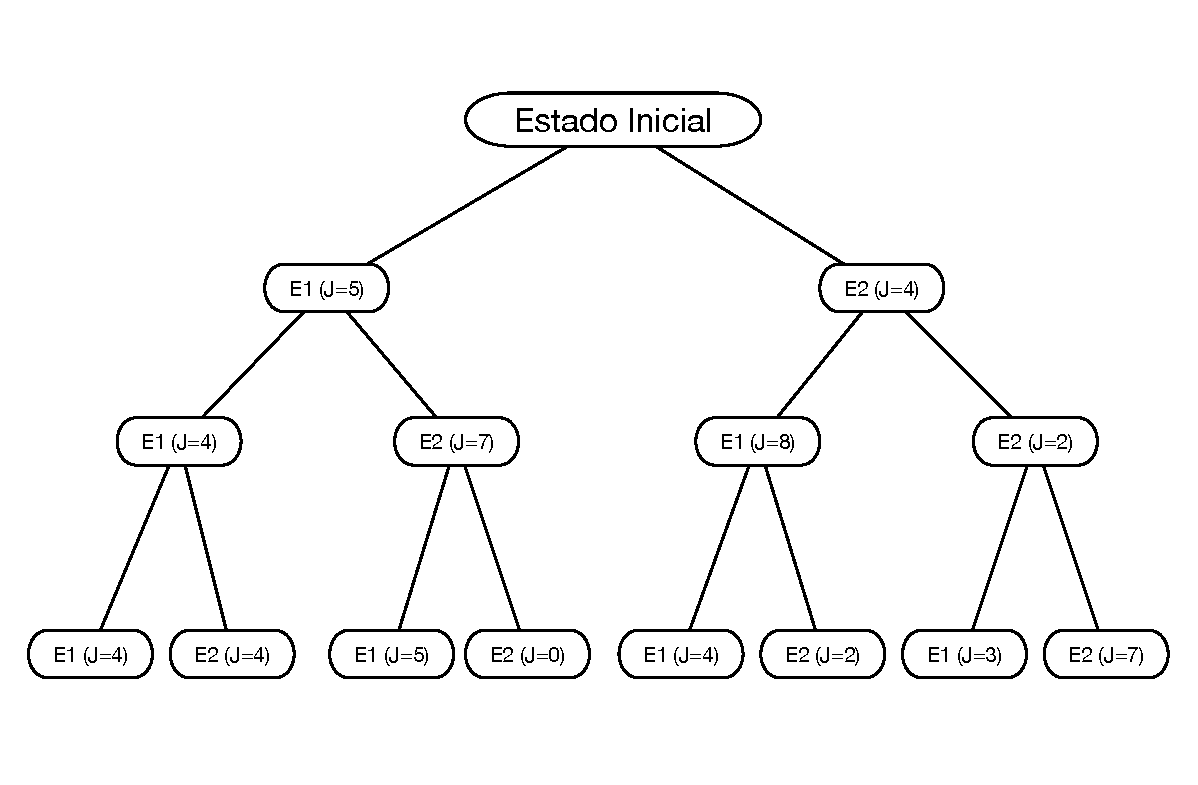
\includegraphics[scale=0.6]{img/planning.eps}
  \caption{Exemplo de \textit{planning} com horizonte 3 e dois elevadores.}
\label{fig:planning}
\end{figure}

O algoritmo é executado (acarretando uma reavaliação) a cada evento do sistema
de simulação, descrito no Capítulo~\ref{chap:modeling}.

\subsection{Função de Custo como Algoritmo de Planning}

Pode-se ver que, para cada etapa do algoritmo de \textit{planning}, estamos
avaliando uma função de custo. Isto fica mais explícito na
figura~\ref{fig:planning}. Considerando este algoritmo com horizonte 1, o
resultado obtido seria idêntico ao de apenas avaliar a função de custo
para uma única tomada de decisão, como proposto na
seção~\ref{sec:ai:minimize-cost-function}. Ou seja, o algoritmo de função de
custo visto anteriormente é apenas um caso especial do descrito aqui.

\section{Planning Multi-Agente}

Este algoritmo é uma extensão do algoritmo de \textit{planning}, onde, em vez de
haver um processamento central que decide que um elevador deve atender a
chamada, tem-se todos os elevadores calculando por conta própria se vale a pena
atender uma chamada ou não.

A literatura neste tópico é ainda escassa. Um estudo deste tipo de comportamento
seria interessante, mas dado o tempo disponível para a implementação e teste,
possivelmente não será viável.

Uma possível implementação deste tipo de algoritmo faria com que cada elevador
avaliasse qual chamada, dentre as disponíveis, ele tomaria para si. Para evitar
que todos cheguem à mesma decisão, políticas de escalonamento podem ser
escolhidas. Por exemplo, coloca-se os elevadores em uma fila circular. O
primeiro elevador da fila roda seu algoritmo e calcula qual chamada deve tomar
para si. Ele vai, então, para o fim desta fila, e o próximo elevador toma a
próxima decisão.

Os algoritmos que cada elevador pode utilizar são as variações de funções de
custo e \textit{planning}, com variações no horizonte.

\section{Políticas de Ociosidade}

Há ainda um outro detalhe a ser considerado, que pode afetar o desempenho do
sistema: o que um elevador deve fazer quando não há chamadas para ele~-~ou~seja,
o elevador está \textbf{ocioso}.

Há várias possibilidades para isto, e é interessante testar-se várias delas e
comparar-se sua eficácia. Por exemplo, uma política ingênua seria manter o
elevador no último andar onde ele parou. Outra política, também bastante
simples, seria mandar todo elevador ocioso de volta para o térreo.

Políticas mais inteligentes podem maximizar a distância entre elevadores
ociosos. Por exemplo, o primeiro elevador ocioso deve ir para o térreo. O
segundo, para o andar mais alto. O terceiro, para um andar intermediário~-~e
assim por diante.

Há ainda a possibilidade de analisar-se os padrões de tráfego. Como sabe-se o
histórico de chegadas de passageiros em cada andar, pode ser tomada a decisão de
mandar elevadores ociosos para os andares onde é mais provável que alguma nova
chamada surja. No entanto, este tipo de comportamento está fora do escopo deste
trabalho, por motivos de limitação de tempo.